\documentclass{beamer}

\usepackage[utf8]{inputenc}
\usepackage[english,ngerman]{babel}

\usepackage[natbib=true,style=numeric,backend=biber,useprefix=true]{biblatex}
\setbeamercolor*{bibliography entry title}{fg=black}
\setbeamercolor*{bibliography entry location}{fg=black}
\setbeamercolor*{bibliography entry note}{fg=black}
\setbeamertemplate{bibliography item}{\insertbiblabel}
\renewcommand*{\bibfont}{\scriptsize}
\addbibresource{kolloquium.bib}

\usepackage{caption}
\captionsetup[figure]{labelformat=empty}

\usetheme{Malmoe}
\usecolortheme{dove}
\usefonttheme{structurebold}

\setbeamertemplate{navigation symbols}{}%remove navigation symbols
\setbeamertemplate{footline}[frame number]{}

\title[HoloLens Anwendung für Windows Mixed Reality]{Augmented Reality Anwendung für Windows Mixed Reality unter Verwendung der HoloLens zur Vermarktung von Werbeflächen}
\date[2017]{Donnerstag, 19. Oktober 2017}
\author[S. Schröder]{Sören Schröder}
\institute[Uni Koblenz]{Universität Koblenz Landau}


\begin{document}
\begin{frame}[plain]
    \maketitle
    \begin{figure}
        \centering
        \begin{minipage}{.5\textwidth}
            \centering
            
\includegraphics[width=.9\linewidth]{logos/UniLogoNeu}
        \end{minipage}%
        \begin{minipage}{.5\textwidth}
            \centering
            
\includegraphics[width=.9\linewidth]{logos/brickmakers-logo}
        \end{minipage}
    \end{figure}   
\end{frame}

\begin{frame}
    \frametitle{Inhalte}
    \setcounter{secnumdepth}{2}
    \tableofcontents[pausesections, hideallsubsections]
\end{frame}

\section{Einleitung}
\begin{frame}
    \frametitle{\insertsection}
    \begin{itemize}[<+->]
        \item AR und VR Lösungen für Konsumenten
        \item Möglich durch Entwicklung der Smartphones
        \item HoloLens
    \end{itemize}

% - Verfügbarkeit von AR und VR Geräten in letzten Jahren gestiegen
% - Thema ist in der breiten Masse angekommen
%   - Beispiele für VR: Cardboard, Oculus
%   - Beispiele für AR: Pokémon Go, AR-Kit Apple
%   - Schlüssel hierfür -> Entwicklung auf dem Markt für Smartphones (Displays (DPI) und Rechenleistung zu geringen Preisen)
% - HoloLens
%   - Wählt Ansatz mit durchsichtigen Displays
%   - Kann virtuelle Objekte mit dem durch Sensoren erfassten Raum interagieren lassen
%   - Erstes frei verkäufliche Gerät dieser Art
\end{frame}

\subsection{Motiviation}
\begin{frame}
    \frametitle{\insertsubsection} 
    \begin{figure}
        \centering
        \begin{minipage}{.5\textwidth}
            \centering
            \includegraphics[width=.9\linewidth]{images/HololensUsecaseCar}
            \caption{Untersstützung bei Arbeiten~\cite{HoloLensVolvo:3ZnwAVSG}}
        \end{minipage}%
        \begin{minipage}{.5\textwidth}
            \centering
            \includegraphics[width=.9\linewidth]{images/HololensUsecaseGame}
            \caption{Neue Spielerfahrungen~\cite{HoloLensFractions:qf6SMVOm}}            
        \end{minipage}
    \end{figure}  


    % - HoloLens bietet mögliche Einsatzgebiete
    %   - Überstützung bei Arbeiten durch einblenden von virtuellen Objekten
    %       - Reparatur von Maschinen
    %   - Neue Spielerfahrung
\end{frame}

\begin{frame}
    \frametitle{\insertsubsection}
    \begin{figure}
        \centering
        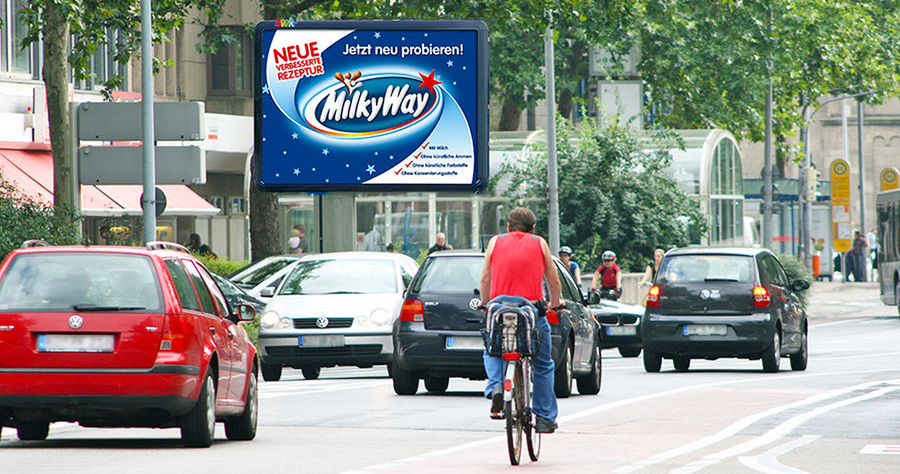
\includegraphics[width=\linewidth]{images/Billboard}
        \caption{Großfläche (Plakatwand) der awk~\cite{GrossflacheStandort:2017vl}\label{fig:Billboard}}
      \end{figure}
\end{frame}

\subsection{Aufgabenstellung}
\begin{frame}
    \frametitle{\insertsubsection}
    \begin{itemize}
        \item Entwicklung eine HoloLens Anwendung
        \item Anwendung zur Vermarktung von Werbeflächen
        \item Grenzen und Möglichkeiten der HoloLens        
    \end{itemize}
    % - Entwicklung einer Anwendung für die Window Mixed Reality Plattform, im speziellen für die HoloLens
    % - Anwendung zur Vermarktung von Werbeflächen
    %   - Anzeigen von Metadaten am Standort
    % - Forschungsfrage: Was sind die Grenzen und Möglichkeiten der HoloLens
\end{frame}

% \section{Grundlagen}
% \begin{frame}
    
% \end{frame}

% \subsection{Reality-Virtuality-Conitnuum}
% \begin{frame}
%     \frametitle{\insertsubsection}  
%     \begin{figure}
%         \centering
%         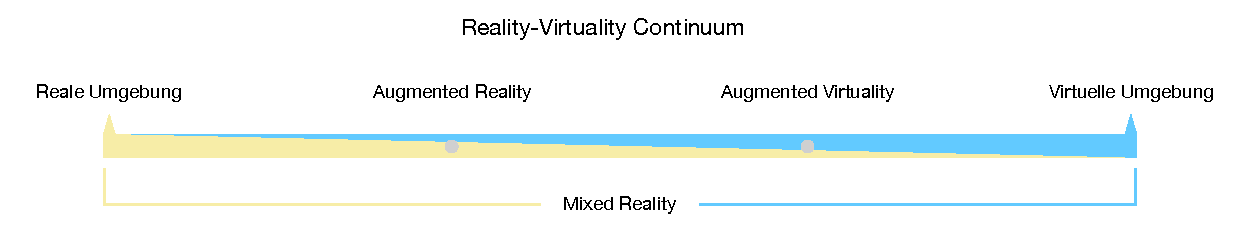
\includegraphics[width=\linewidth]{images/RVC}
%         \caption{Reality-Virtuality Conitnuum nach Milgram et al. (1994)~\cite{Milgram:1994vl}}
%     \end{figure}
% \end{frame}

% \begin{frame}
%     \frametitle{Augmented Reality}
%     \begin{figure}
%         \centering
%         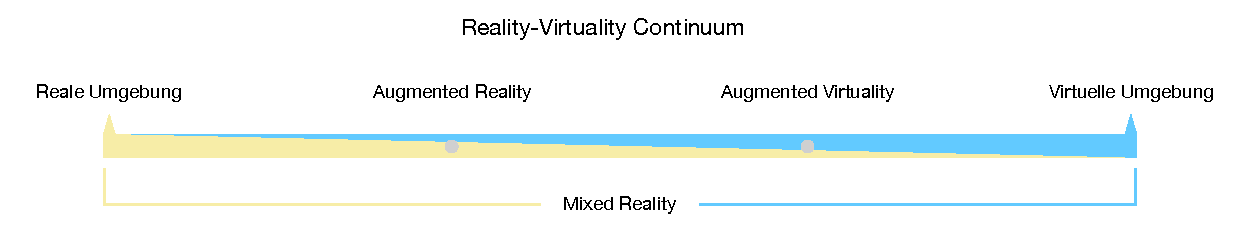
\includegraphics[width=\linewidth]{images/RVC}
%         \caption{Reality-Virtuality Conitnuum nach Milgram et al. (1994)~\cite{Milgram:1994vl}}
%     \end{figure}

%     % - AR: Erweitern der Realität
%     %   - Mehr Realität als virtuelle Elemente
%     %   - Realität wird angereichert
% \end{frame}

% \begin{frame}
%     \frametitle{Augmented Reality}

%     \begin{figure}
%         \centering
%         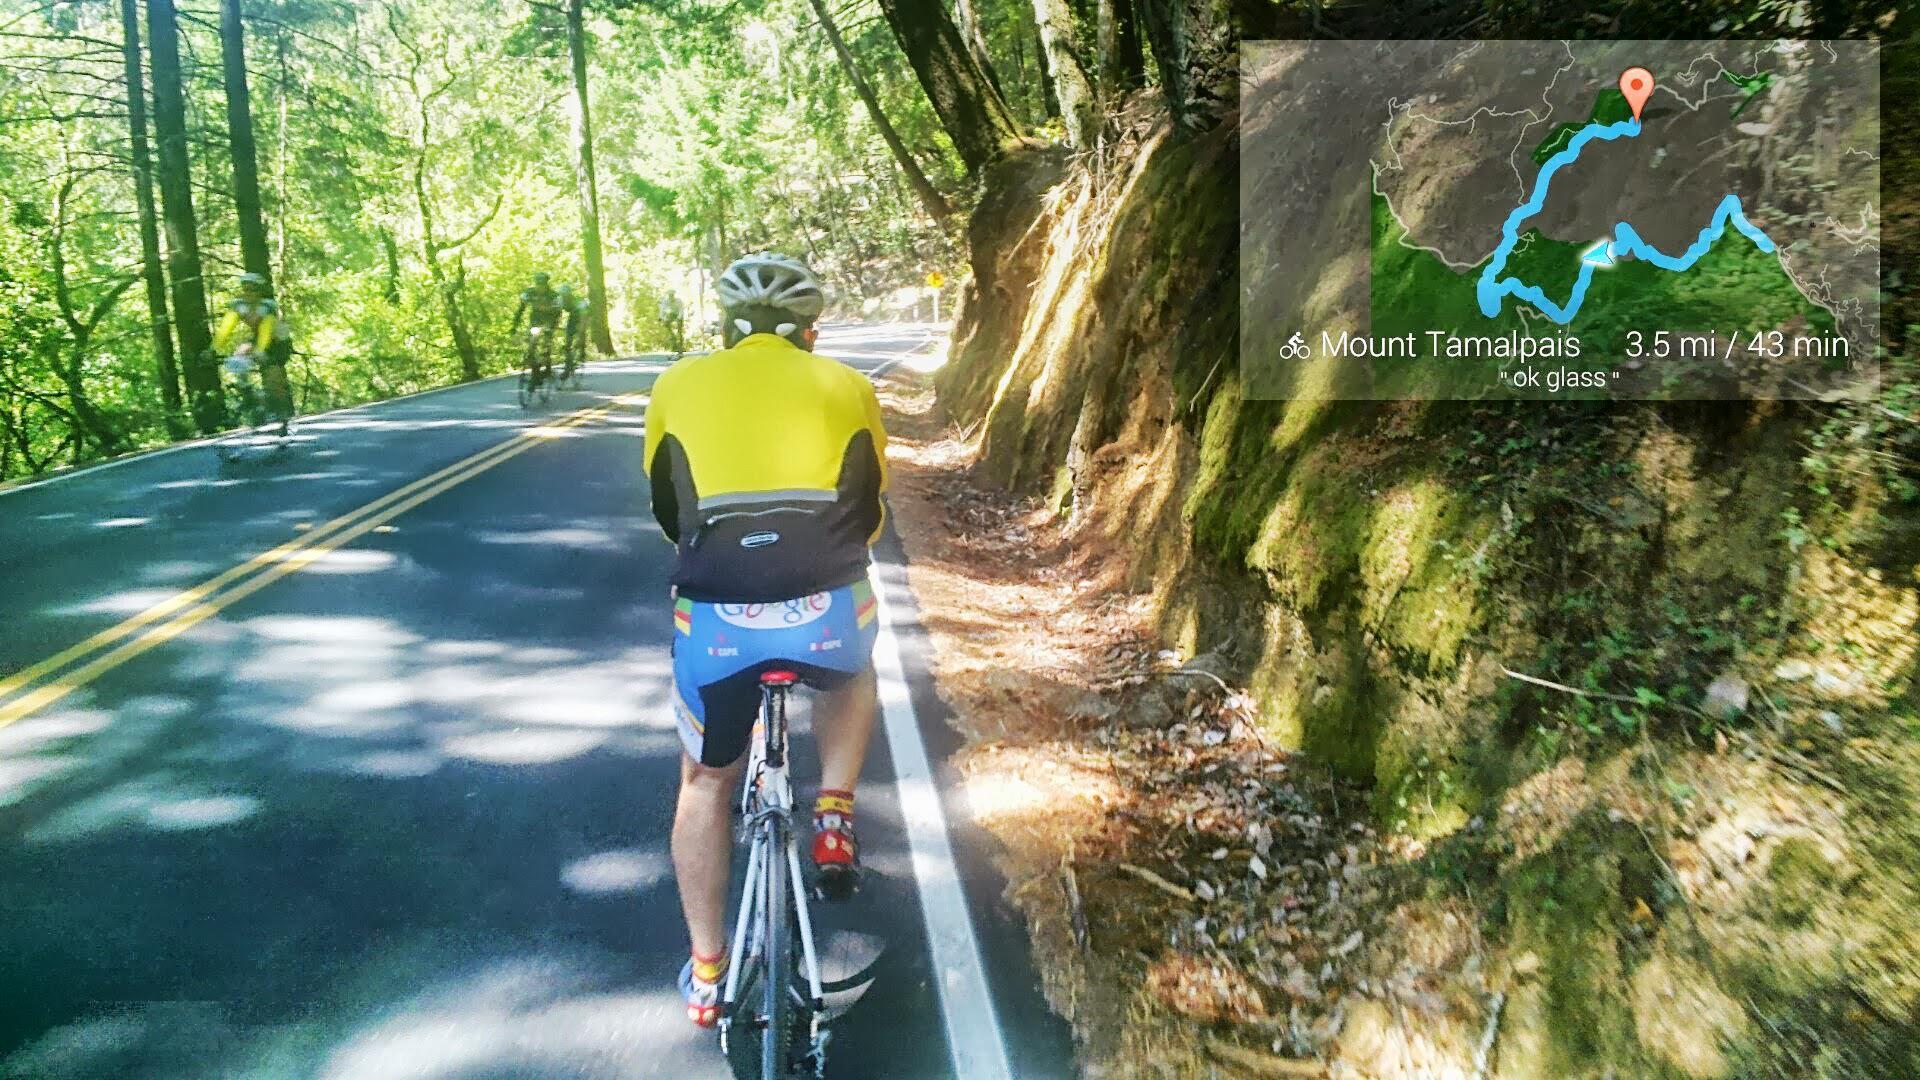
\includegraphics[width=.6\linewidth]{images/GlassNavigation}
%         \caption{Google Glass Navigation~\cite{GoogleGlassNavigat:PyBuqepU}}
%     \end{figure}

%     % - AR: Erweitern der Realität
%     %   - Beispiel Google Glass
%     %   - Weiteres Pokémon Go
% \end{frame}

% \begin{frame}
%     \frametitle{Augmented Virtuality}  
%     \begin{figure}
%         \centering
%         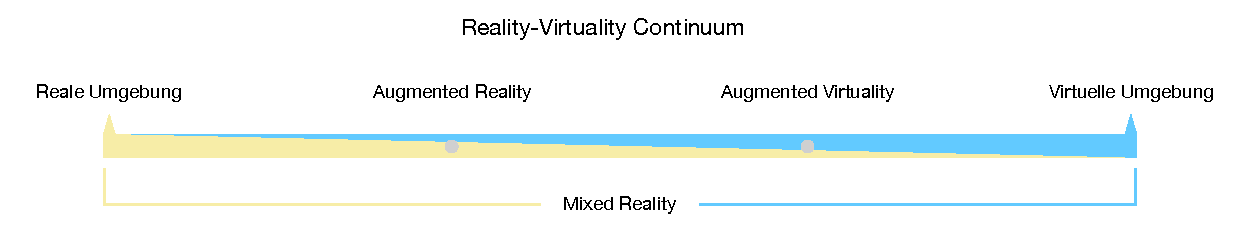
\includegraphics[width=\linewidth]{images/RVC}
%         \caption{Reality-Virtuality Conitnuum nach Milgram et al. (1994)~\cite{Milgram:1994vl}}
%     \end{figure}

%     % - AV: Erweitern der Virtualität
%     %   - Mehr Virtuelles als Reales
%     %   - Virtuelle Szene wird mit realen Inhalten angereichert
% \end{frame}

% \begin{frame}
%     \frametitle{Augmented Virtuality}  
    
%     \begin{figure}
%         \centering
%         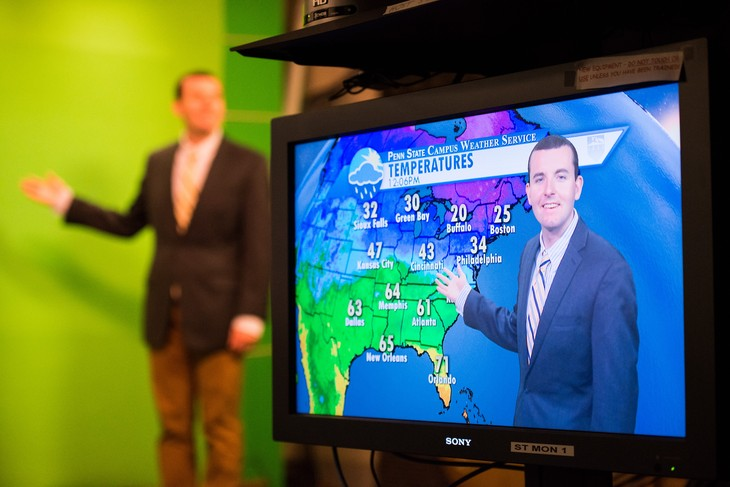
\includegraphics[width=.7\linewidth]{images/weather}
%         \caption{Aufzeichnung eines Wetterberichts~\cite{WeatherForcastCWS:vz}}
%     \end{figure}

%     % - AV: Erweitern der Virtualität
%     %   - Beispiel Wetterkarte
%     %   - RVC auch auf nicht stereoskopische Lösungen anwendbar
% \end{frame}


% \begin{frame}
%     \frametitle{Virtual Reality}  
%     \begin{figure}
%         \centering
%         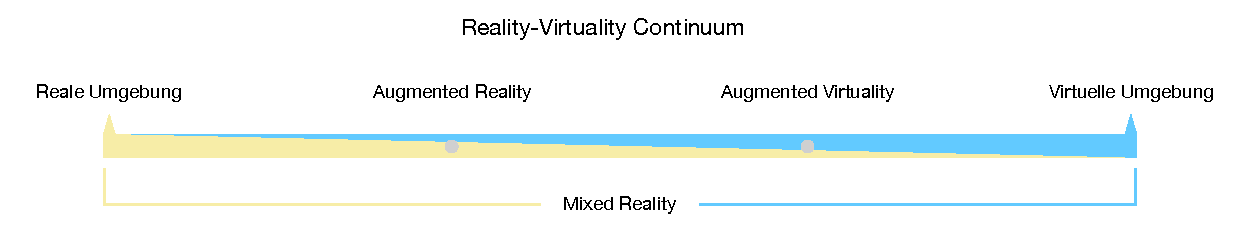
\includegraphics[width=\linewidth]{images/RVC}
%         \caption{Reality-Virtuality Conitnuum nach Milgram et al. (1994)~\cite{Milgram:1994vl}}
%     \end{figure}

%     % - VR: Virtuelle Realität
%     %   - Beispiel Oculus
%     %   - Unterschied zwischen VR und virtueller Umgebung
% \end{frame}

% \begin{frame}
%     \frametitle{Mixed Reality}  
%     \begin{figure}
%         \centering
%         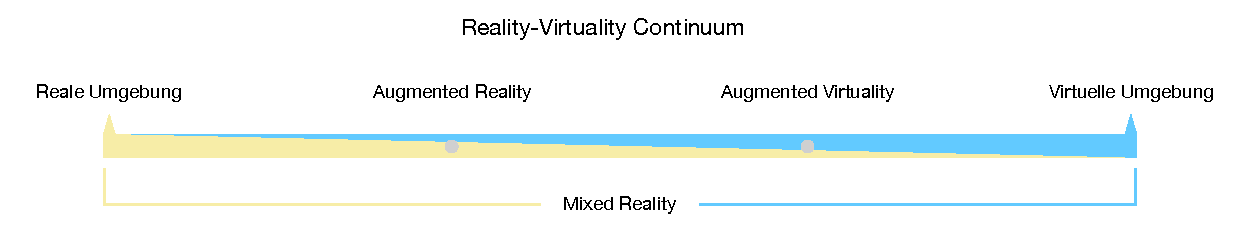
\includegraphics[width=\linewidth]{images/RVC}
%         \caption{Reality-Virtuality Conitnuum nach Milgram et al. (1994)~\cite{Milgram:1994vl}}
%     \end{figure}

%     % - MR: Mixed Reality
%     %   - Gseamtbereich des RVC
%     %   - Übergänge zwischen den einzelnen Definitionen sind fließend Reality -> AR -> AV -> VR -> Virtuality (Matrix)
% \end{frame}

% \subsection{Mixed Reality Plattform}
% \begin{frame}
%     \frametitle{Mixed Reality Plattform}  
%     \begin{figure}
%         \centering
%         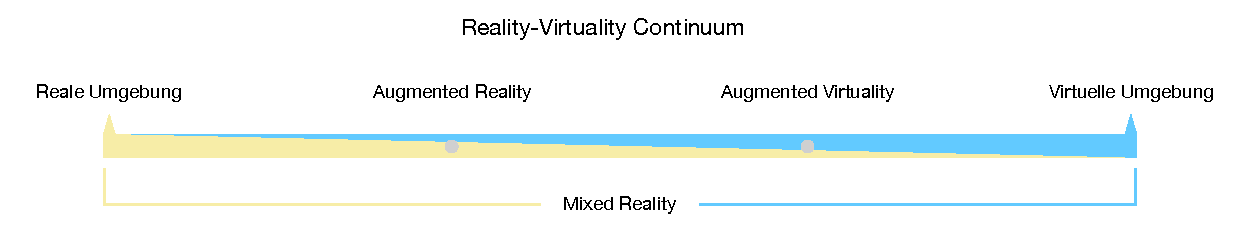
\includegraphics[width=\linewidth]{images/RVC}
%     \end{figure}

%     \begin{figure}
%         \centering
%         \begin{minipage}{.5\textwidth}
%             \centering
%             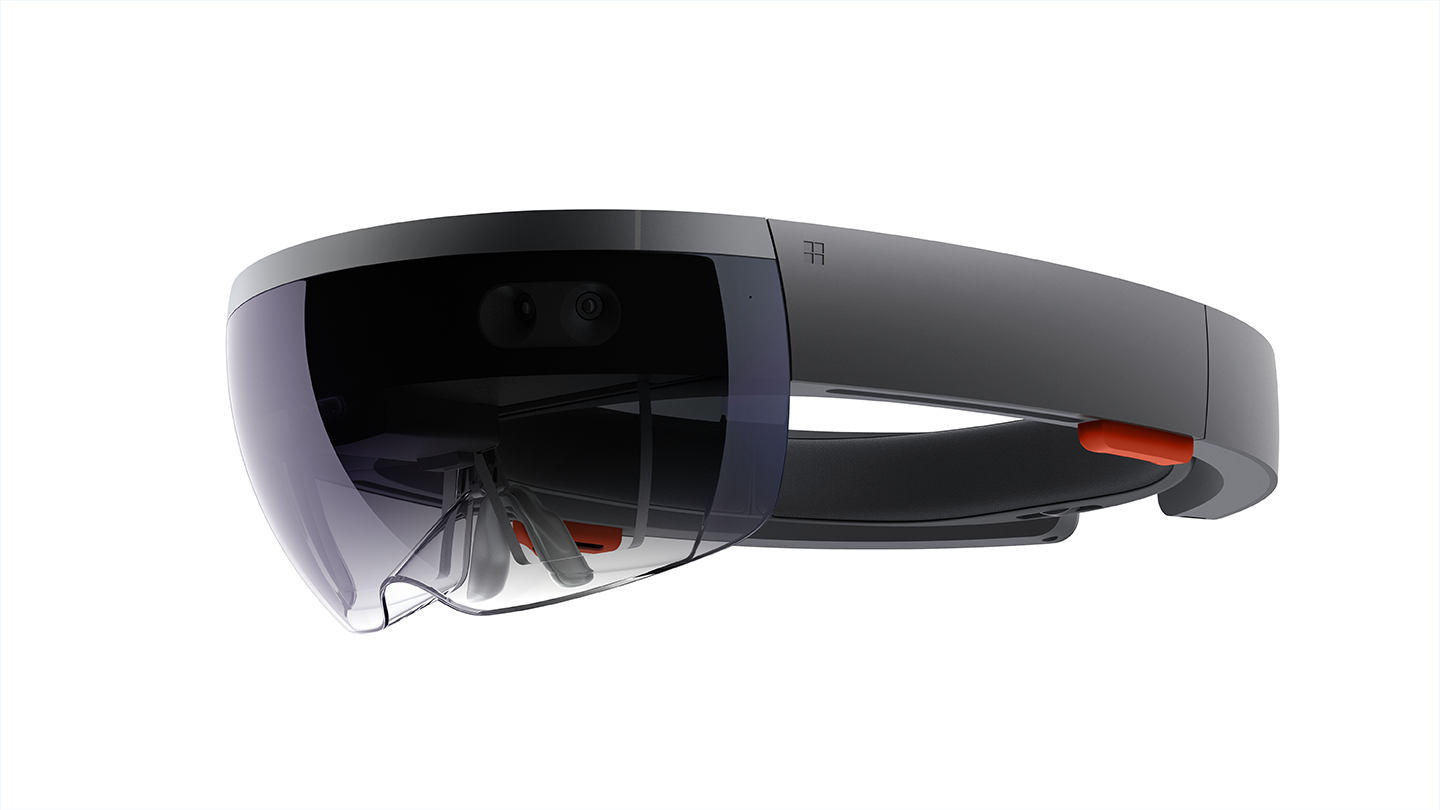
\includegraphics[width=.9\linewidth]{images/HoloLens}
%             \caption{Holographisches Gerät~\cite{HoloLens:uH2UA4Mc}}
%         \end{minipage}%
%         \begin{minipage}{.5\textwidth}
%             \centering
%             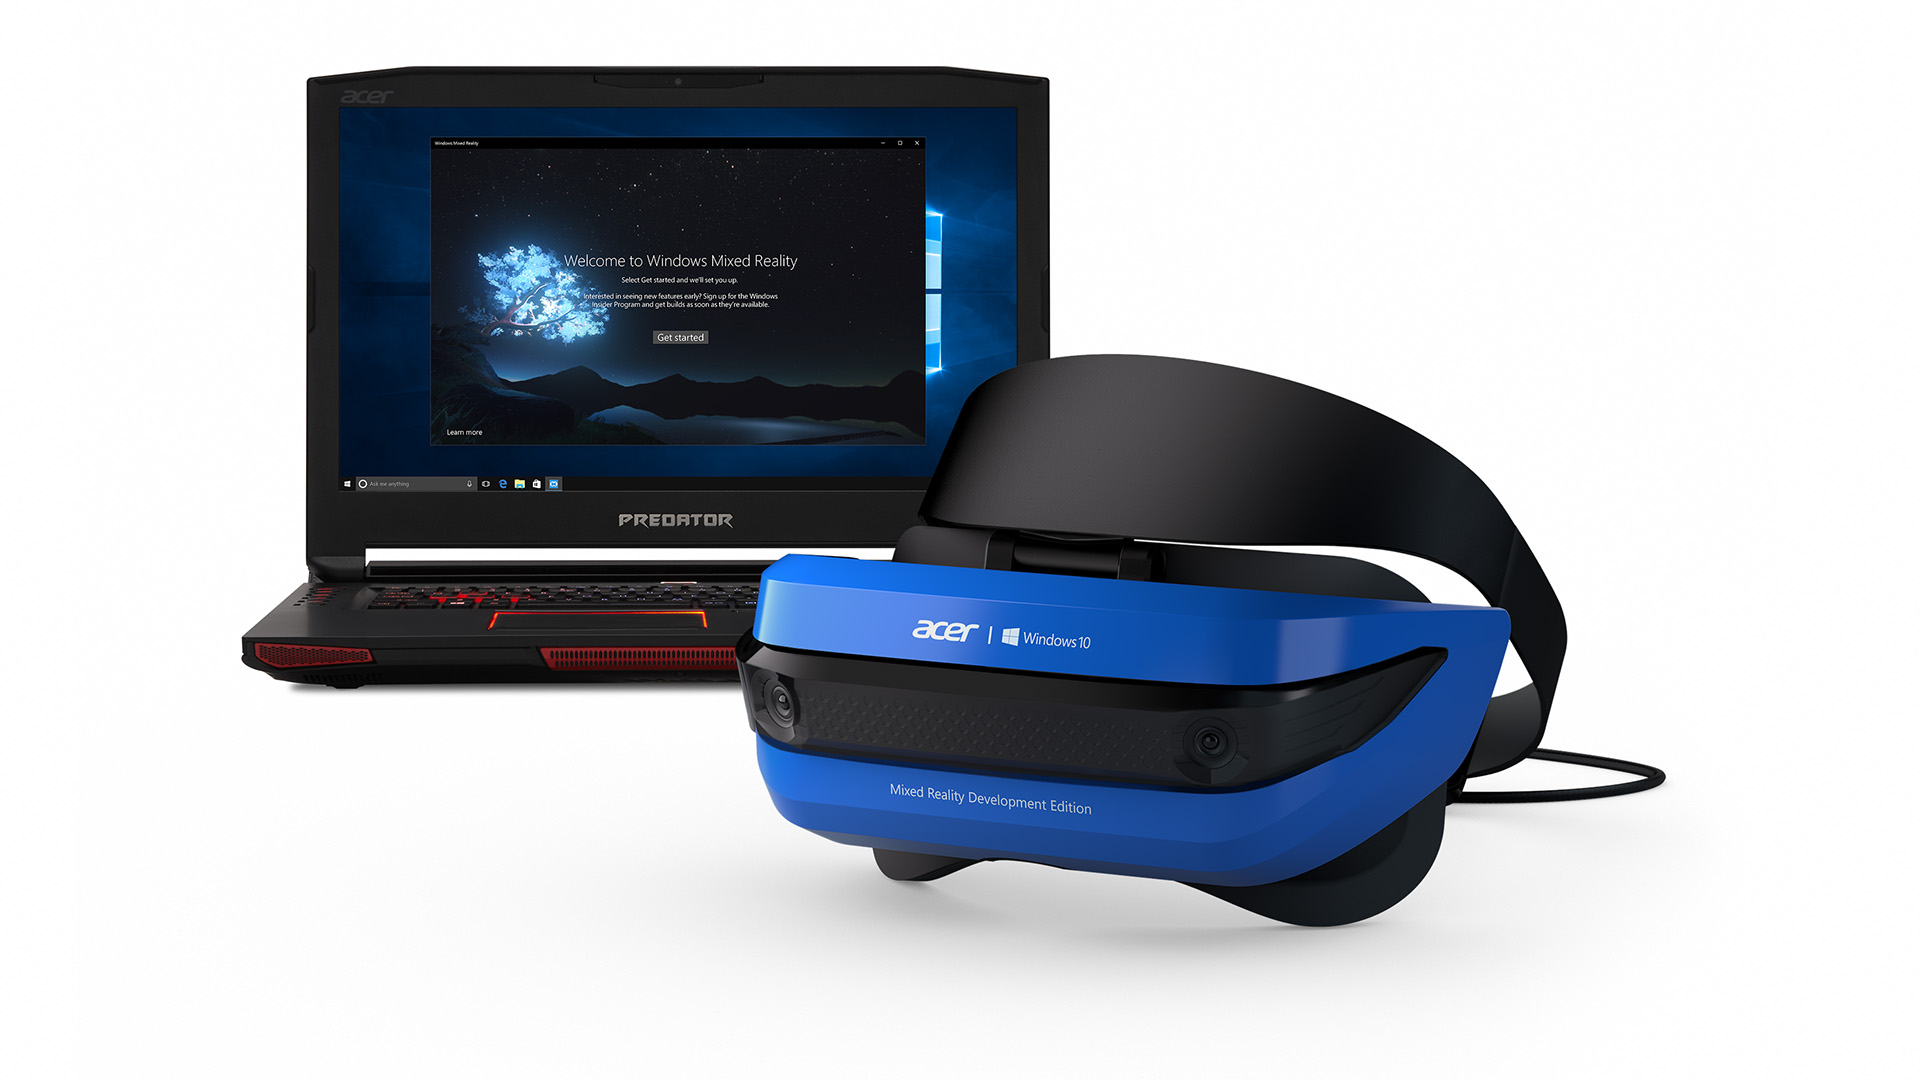
\includegraphics[width=.9\linewidth]{images/AcerMixedReality}
%             \caption{Immersives Gerät~\cite{AcerWindowsMixedR:mJmOAe22}}
%         \end{minipage}
%     \end{figure} 

%     % - Plattform von Microsoft zur Vermischung der physikalischen mit virtuellen Welten
% \end{frame}

% \begin{frame}
%     \frametitle{Mixed Reality Plattform}  

%     % - Plattform von Microsoft zur Vermischung der physikalischen mit virtuellen Welten
%     % - Zwei Geräteklassen
%     %   - Holographische Geräte (transparente Displays)
%     %   - Immersive Geräte  (opake Displays)
% \end{frame}

\section{Microsoft HoloLens}

\begin{frame}
    \frametitle{\insertsection}
    \begin{figure}
        \centering
            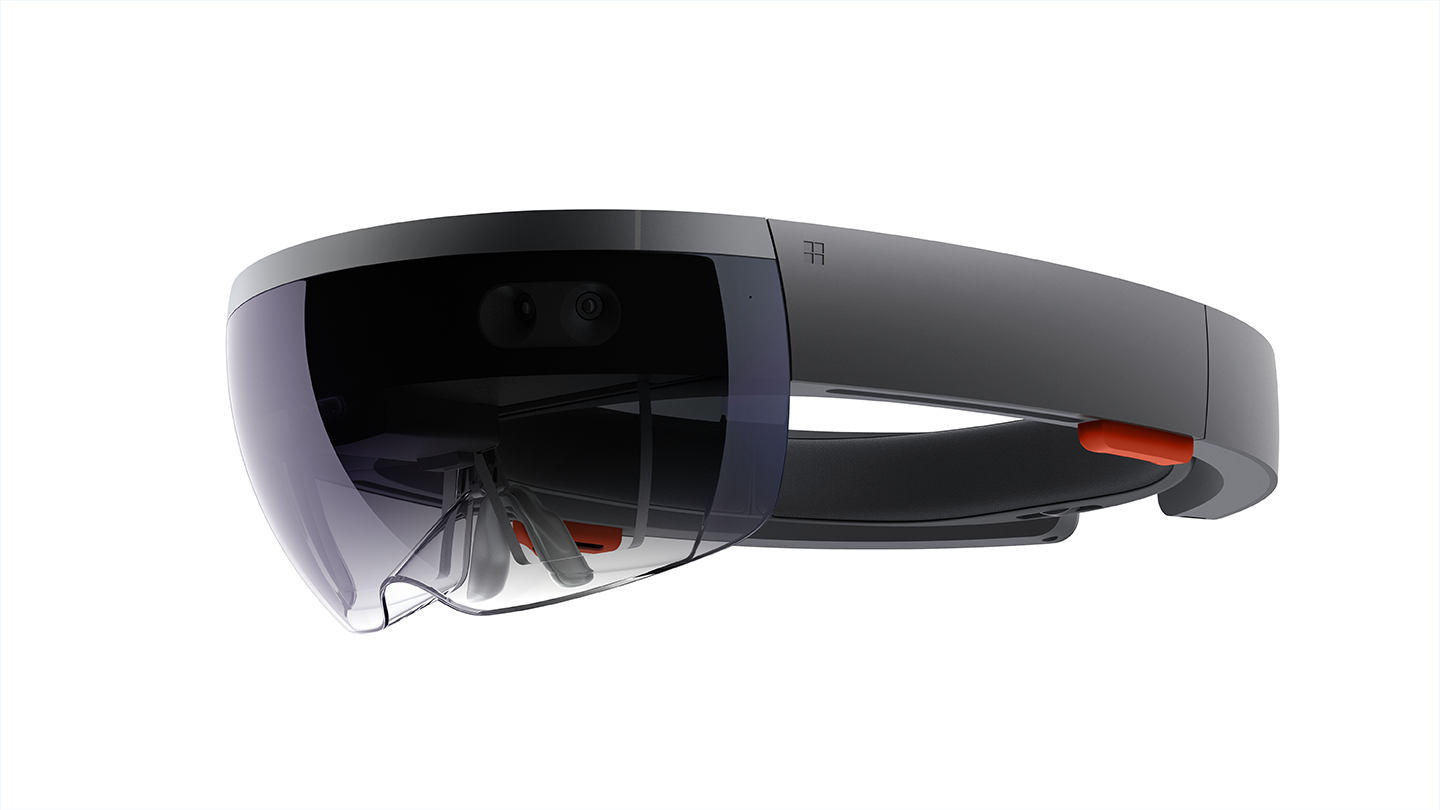
\includegraphics[width=.9\linewidth]{images/HoloLens}
            \caption{Microsoft HoloLens~\cite{HoloLens:uH2UA4Mc}}
      \end{figure}
    % - Unterschied zwischen AR Geräten und HoloLens deutlich machen
    %   - Erkennung des Raums
    %   - Interaktion von virtuellen Elementen mit dem Raum
    %   - Bestimmung der Pose mit Inside Out Tracking
    % - Teile der Hardware ähnlich zu anderen mobilen Computer (Bspw. Intel Atom CPU, RAM, Batterie usw.)
\end{frame}

\begin{frame}
    \frametitle{\insertsection}
    \begin{figure}
        \centering
        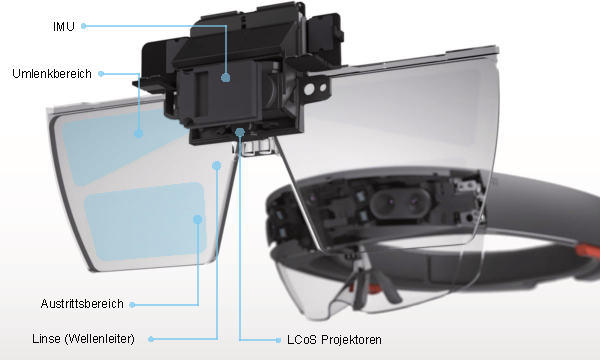
\includegraphics[width=.8\linewidth]{images/HoloLensOptics}
          \caption{Optik der HoloLens~\cite{Microsoft:ug}~\cite{Colaner:2016to}}
      \end{figure}
    % - IMU Gyroskop, Magnetometa, Beschleunigungsmesser
    % - Projektoren werfen Bild in Linse (Wellenleiter)
    % - Licht wird durch entsprechende optische Gitter gebrochen -> Totalreflexion
    % - Licht wird durch Umlenkbereich Richtung Austrittsbereich gelenkt.
    % - Licht tritt aus -> Bild auf Display 
\end{frame}

\begin{frame}
    \frametitle{\insertsection}
    \begin{figure}
        \centering
        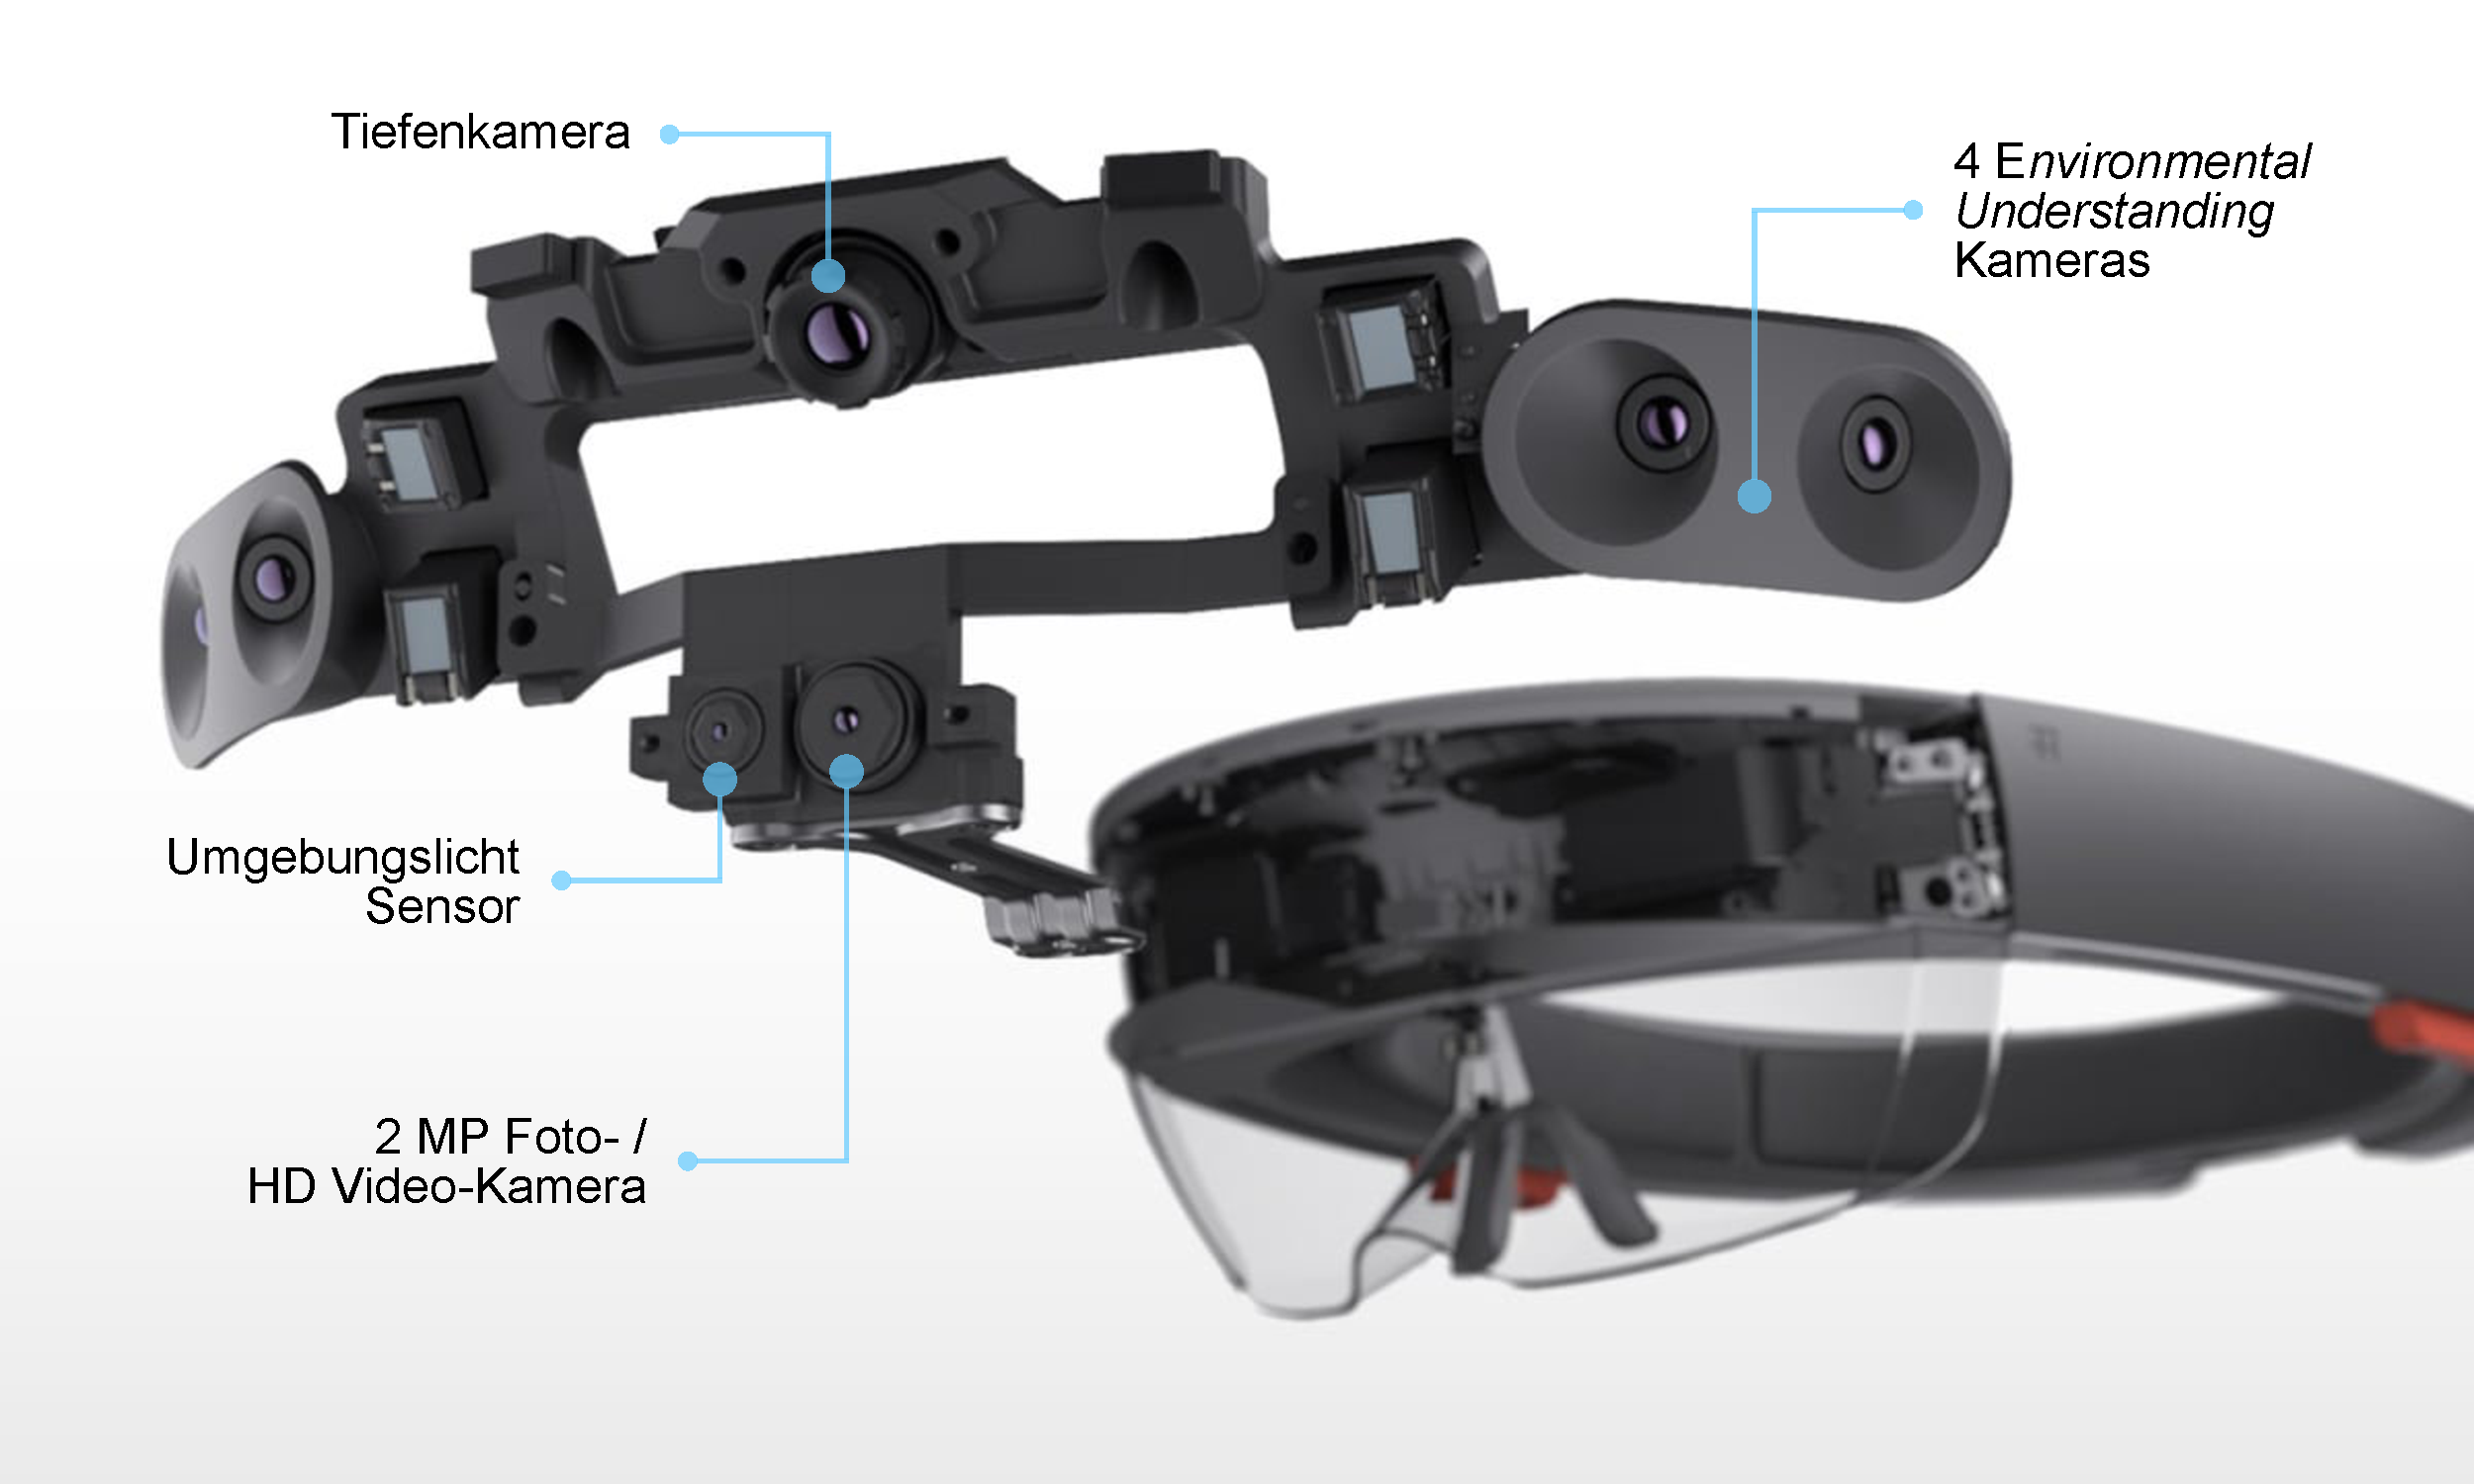
\includegraphics[width=.8\linewidth]{images/HoloLensCameras}
          \caption{Sensorleiste der HoloLens~\cite{Microsoft:tn}~\cite{Colaner:2016to}}
      \end{figure}
    % - Webcam: Aufnahme von Bildern und Videos
    % - Umgebungslichtsensor: Helligkeitsanpassung
    % - Tiefenkamera: Umgebungserkennung mittels Infrarotlicht Erkennung (Infrarotlicht von eigenen Projektoren)
    %   - ( ToF (Time of Flight) Puls oder Sinusmodulation)
    % - Environmental Understanding Kameras: Position im Raum und Gestenerkennung (Tiefenkamer unterstützt)

\end{frame}

\section{Konzeption}
\subsection{Anwendungsszenario}
\begin{frame}
    \frametitle{\insertsubsection}
    \begin{itemize}[<+->]
        \item Kunde betrachtet Plakatwände vor Ort
        \item Anwendung ermöglicht Anzeige von Informationen
    \end{itemize}
    % - Kunde schaut sich Plakatwände vor Ort an
    % - Anwendung zeigt ihm aktuelle Informationen zur entsprechenden Plakatwand and
    %   - Preis, Verfügbarkeit, Personenkontakte 
    % - Informationen können vom Nutzer ein und ausgeblendet werden
\end{frame}

\subsection{Anforderungen}
\begin{frame}
    \frametitle{\insertsubsection}
    \begin{itemize}[<+->]
        \item Identifizierung der Plakatwand
        \item Anforderung der Informationen
        \item Anzeige der Informationen  
        \item Eindeutige Zuordnung zu Plakatwand
        \item Ausblenden der Informationen
        \item Aktualität der Informationen
    \end{itemize}
    % - Die Anwendung muss die Plakatwand, zu der Informationen angefordert werden, identifizieren.
    % - Der Benutzer hat die Möglichkeit Informationen zu einer Plakatwand anzufordern.
    % - Der Nutzer muss wissen, für welche Plakatwand er Informationen angezeigt bekommt.
    % - Die Informationen müssen dem Benutzer angezeigt werden.
    % - Der Benutzer hat die Möglichkeit die Informationen auszublenden.
    % - Für den Benutzer muss jederzeit erkennbar sein, wo die Informationen angezeigt werden.
    % - Die angezeigten Informationen müssen nach Änderungen seitens des Anbieters beim nächsten Anzeigen aktualisiert sein.
\end{frame}

\section{Lösungsanstäze}
\subsection{Identifizierung der Plakatwand}
\begin{frame}
    \frametitle{\insertsubsection}
    \begin{figure}
        \centering
        \begin{minipage}{0.74\linewidth}
            \centering
            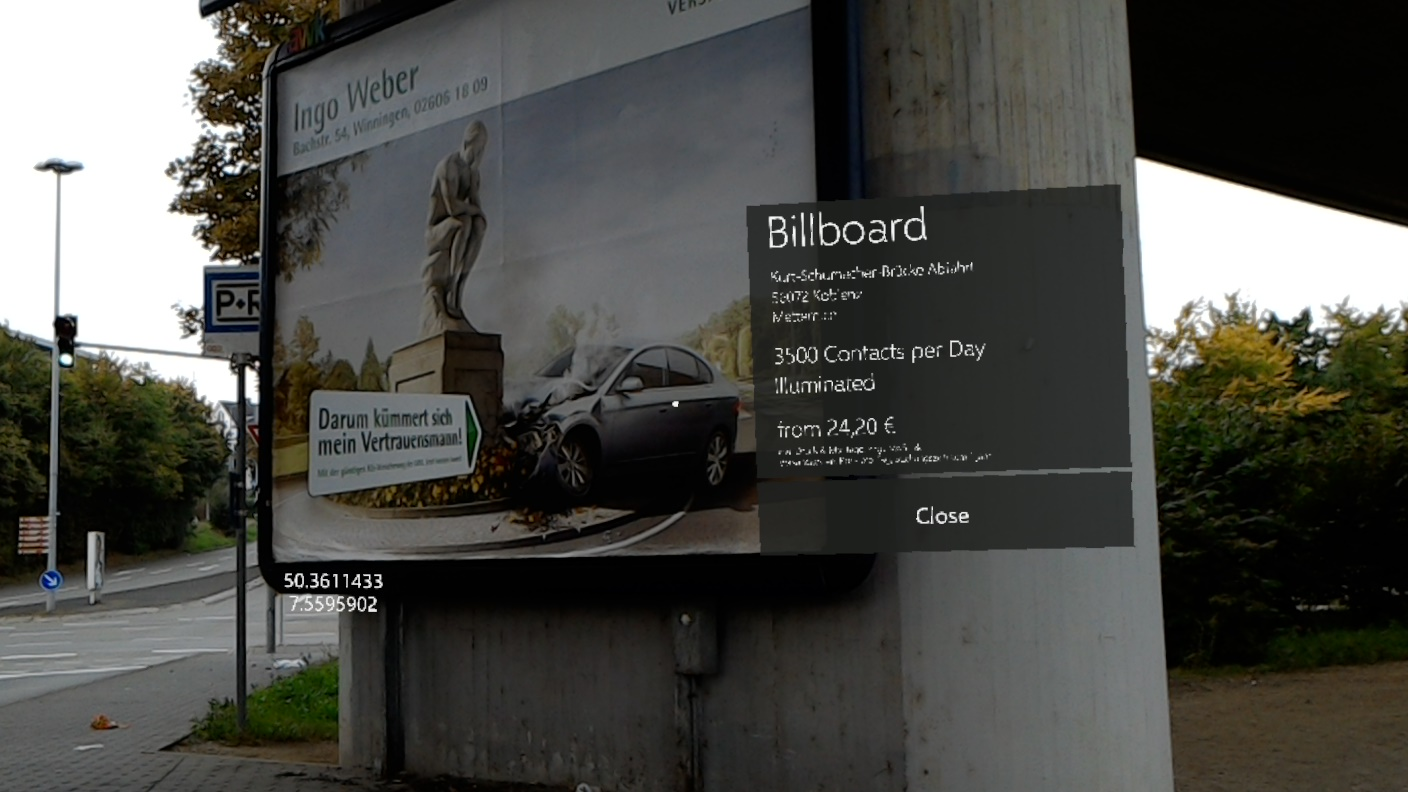
\includegraphics[width=\linewidth]{images/UIWithGeolocation1}
        \end{minipage}%
        \begin{minipage}{0.24\linewidth}
            \centering
            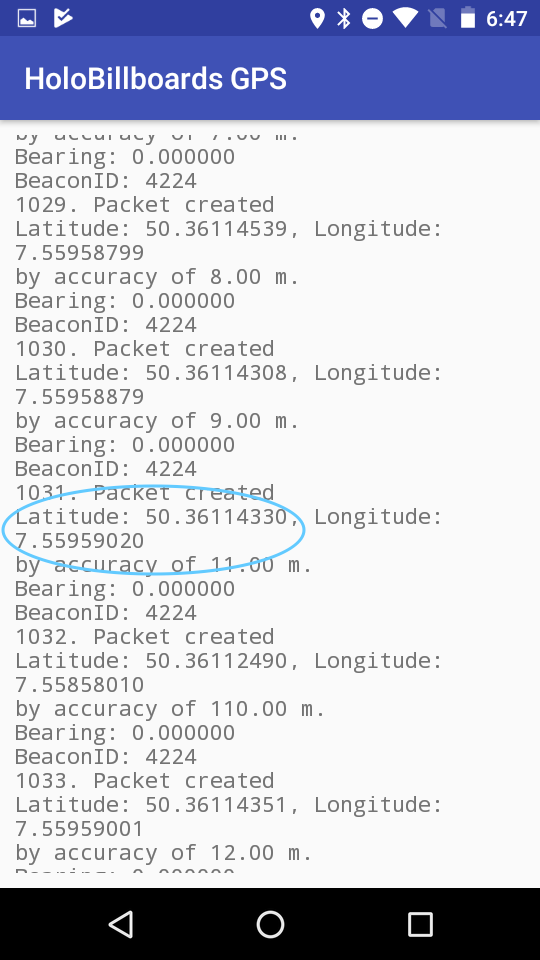
\includegraphics[width=\linewidth]{images/GPSLog}        
        \end{minipage}
    \end{figure}

    % - Bestimmen des Standortes des Nutzers mittels GPS notwendig
    %   - HoloLens besitzt kein GPS
    %   - Positionsbestimmung am Smartphone
    %   - Übermittlung per Bluetooth LE Advertising
    %       - Keine Kopplung der Geräte Notwendig
    %       - Identifikation der Pakte über Manufacturing ID
    %       - Pakete können abgefangen und falsche Pakete empfangen werden -> Beides kein signifikantes Problem
\end{frame}

\subsection{Anfordern der Informationen}
\begin{frame}
    \frametitle{\insertsubsection}
    \begin{figure}
        \centering
        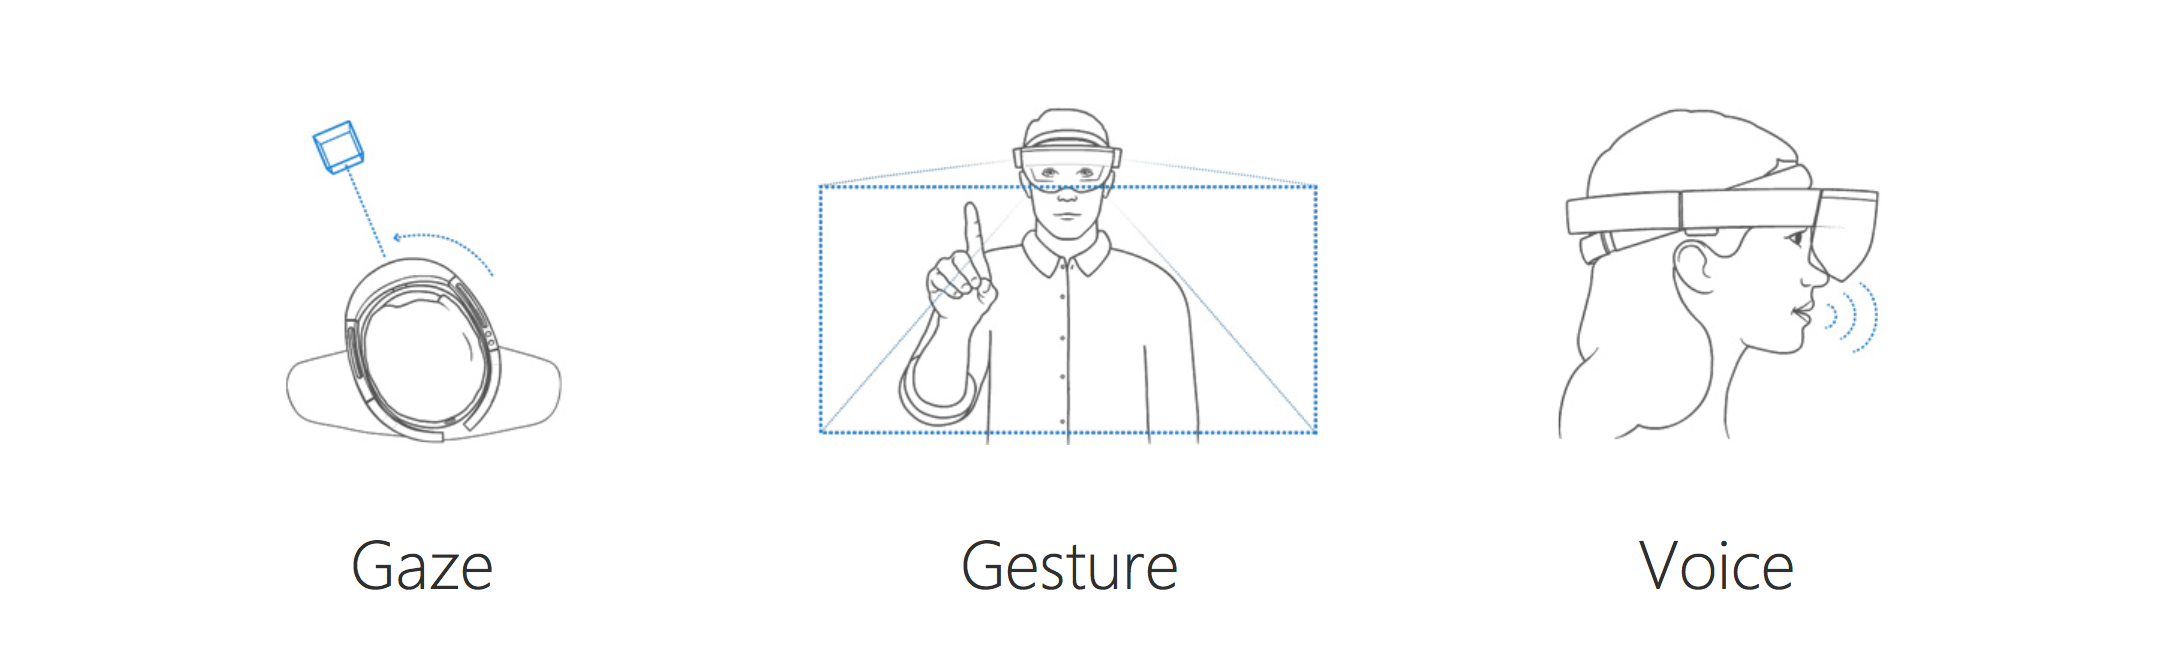
\includegraphics[width=\linewidth]{images/Interaction}
        \caption{Interaktion mit der HoloLens~\cite{HoloLensInteraction:IaH8RfEh}}
    \end{figure}
    % - Eingabemethoden der HoloLens
    %   - Gaze (Blickrichtung) -> Bestimmt Position des Cursors
    %   - Gesten
    %       - Air Tap analog zu Mausklick
    %       - Bloom Beenden von Anwendungen
    %   - Sprache

    % - In HoloBillboards
    % - Air Tap zum Anfordern der Informationen und Ausblenden Der Informationen
    % - Sprachbefehle zum Ein- und Ausblenden der Informationen
\end{frame}

\subsection{Anzeigen der Informationen}
\begin{frame}
    \frametitle{\insertsubsection}
    \begin{figure}
        \centering
        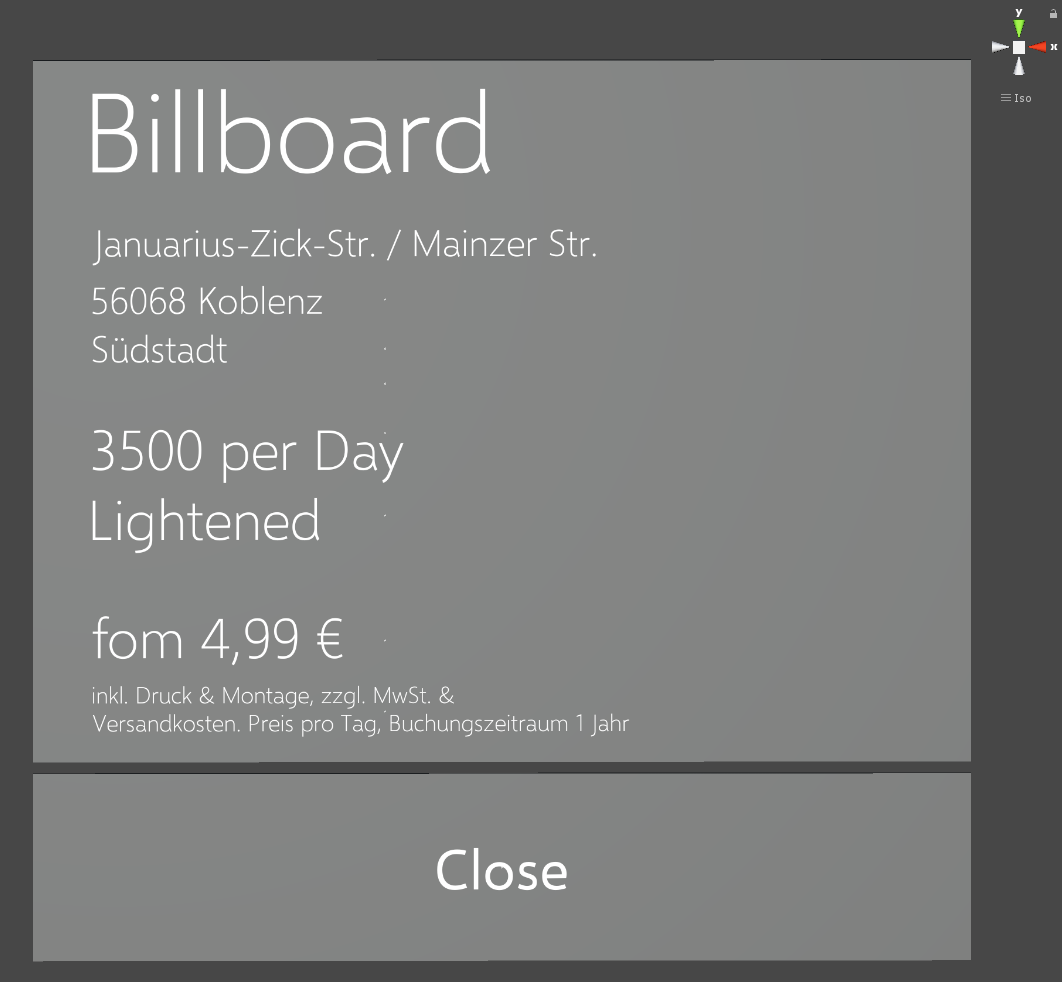
\includegraphics[width=.6\linewidth]{images/DetailWindowInUnity}
    \end{figure}
    % - UI in Unity
    %   - Daten werden in Fenster dargestellt
\end{frame}

\subsection{Eindeutige Zuordnung}
\begin{frame}
    \frametitle{\insertsubsection}
    \begin{figure}
        \centering
        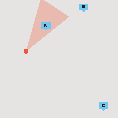
\includegraphics[width=.6\linewidth]{images/billboard_identification_1}
    \end{figure}
    % - Zuordnung zum jetzigen Zeitpunkt implizit über geringsten Abstand möglich
\end{frame}

\subsection{Aktualität der Informationen}
\begin{frame}
    \frametitle{\insertsubsection}
    
\end{frame}

\section{Auswertung}
\begin{frame}
    Lorem Ipsum
\end{frame}

\section{Fazit und Ausblick}
\begin{frame}
    Lorem Ipsum
\end{frame}

\begin{frame}
    \frametitle{Identifizierung der Plakatwand}
    \begin{figure}
        \centering
        \begin{minipage}{.5\textwidth}
            \centering
            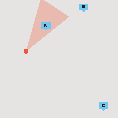
\includegraphics[width=.9\linewidth]{images/billboard_identification_1}
        \end{minipage}%
        \begin{minipage}{.5\textwidth}
            \centering
            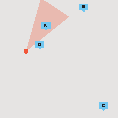
\includegraphics[width=.9\linewidth]{images/billboard_identification_2}
        \end{minipage}
    \end{figure}  
\end{frame}

\begin{frame}
    \frametitle{Identifizierung der Plakatwand}
    \begin{figure}
        \centering
        \begin{minipage}{.5\linewidth}
            \centering
            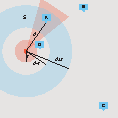
\includegraphics[width=.9\linewidth]{images/billboard_identification_3}
        \end{minipage}%
        \begin{minipage}{.5\linewidth}
            \centering
            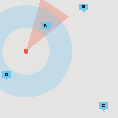
\includegraphics[width=.9\linewidth]{images/billboard_identification_4}       
        \end{minipage}
    \end{figure} 
\end{frame}

\begin{frame}
    \frametitle{Fragen und Diskussion}
    Danke für Ihre Aufmerksamkeit!
\end{frame}

\begin{frame}[allowframebreaks]
    \frametitle{Quellen}
    \printbibliography{}    
\end{frame}

\end{document}